
\begin{problem}{중화요리}
	{standard input}{standard output}
	{1.5초}{64MB}{}
	
	K 이사장을 포함한 정보올림피아드일본위원회의 $N$ 명 모두가 중화요리점에 갔다.
	
	중화요리점의 식탁은 원탁이며, $N$ 명의 자리가 같은 간격으로 떨어져 있다. 또한, 중앙에 요리가 위치한 회전대가 놓여있다. $N$ 명의 위원은 $N$개의 자리에 앉아 있으며, K 이사장을 1번으로 해서 반시계방향으로 $2, 3, \cdots, N$의 위원 번호가 붙어있다. 위원회는 $N$ 종류의 요리를 하나씩 주문해 각 요리를 회전대 위에 올렸다. 각 요리는 각 위원의 앞에 있으며, $i$ 번 위원의 앞에 위치한 요리는 $i$ 번 요리이다. K이사장 이외의 위원은 먹고 싶은 요리가 하나씩 정해져 있고, $i$ 번 ($2 \le i \le N$) 위원이 먹고 싶은 요리는 $A_i$번 요리이다.
	
	회전대는 $(360/N)^{\circ}$ 단위로 시계방향 혹은 반시계방향 어느 방향으로도 회전할 수 있다. 예를 들어, 회전대를 반시계방향으로 한 단위만큼 회전시키면, K 이사장에 앞에는 $N$ 번 요리가, $i$ 번 ($2 \le i \le N$) 위원 앞에는 $i-1$ 번 요리가 온다.
	
	어떤 위원이 어떤 요리를 먹기 위해서는 그 요리가 그 위원의 앞에 오도록 회전대를 돌려야 한다.
	
	정보올림피아드일본위원회에서 K 이사장은 존경받고 있기 때문에, 처음에 K 이사장이 회전대를 회전해서 $k$ 번 ($1 \le k \le N$) 요리가 앞에 오도록 해서 요리를 먹는다.
	
	K 이사장이 요리를 먹은 이후 K 이사장 이외의 위원들은 각각 자신이 먹고 싶은 요리가 앞에 오도록 회전대를 돌려서 그 요리를 먹는다. 단, K 이사장 이외의 위원이 회전대를 돌리는 순서는 어떤 순서여도 상관없다.
	
	또한, 각 요리는 충분히 많기 때문에 요리가 바닥나는 경우는 없다고 한다.
	
	K 이사장이 어떤 요리를 먹어도 상관없도록, 모두가 요리를 먹을 수 있게 회전대를 돌리는 횟수의 합이 최소가 되도록 K 이사장 이외의 위원이 회전대를 돌리는 순서를 각 $k$에 대해서 정해두고 싶다.
	
	$i$ 번 위원이 먹고 싶어 하는 요리의 번호 $A_i$가 각각 주어졌을 때, K 이사장이 먹는 $k$ 번 요리 ($1 \le k \le N$) 각각에 대해 회전대를 돌리는 횟수의 최솟값을 구하여라. 회전대를 $(360/N)^{\circ}$ 돌리는 것을 한 번 돌린다고 한다.


\Constraints


\begin{tabular}{ll}
	$2 \le N \le 100\ 000$ & 정보올림피아드일본위원회의 사람 수 \\
	$1 \le A_i \le N$ & $i$ 번 위원이 먹고 싶은 요리 \\
\end{tabular}


\InputFile

다음 정보가 표준 입력으로 주어진다.

\begin{itemize}
	\item 첫째 줄에는 정수 $N$이 주어지며, 정보올림피아드일본위원회의 사람 수를 의미한다.
	\item 다음 $N-1$ 개의 줄에는 각 위원이 먹고 싶은 요리의 정보가 주어진다. $i$ 번째 ($2 \le i \le N$) 줄에는 정수 $A_i$가 주어진다. 이는 $i$ 번 위원이 먹고싶은 요리가 $A_i$ 번 요리라는 것을 의미한다.
\end{itemize}



\OutputFile

출력은 $N$ 개의 줄로 되어있다. $k$ 번째 ($1 \le k \le N$) 줄에는 K이사장이 $k$ 번 요리를 먹었을 때, 회전대를 돌리는 횟수의 최솟값을 의미하는 정수를 출력하여라. 단, 회전대의 회전량은 $(360/N)^{\circ}$ 돌리는 것을 한 번으로 생각한다.

\Scoring

채점 데이터 중, 배점의 10\%에 대해 $N \le 10$을 만족한다.

채점 데이터 중, 배점의 40\%에 대해 $N \le 1\ 000$을 만족한다.

\Examples

\begin{example}
	\exmp{
		5
		3
		5
		3
		2
	}{%
		4
		4
		5
		6
		4
	}%
\end{example}

이 예에서, 원탁에 5명의 위원이 그림과 같이 앉아있다.

\begin{center}
	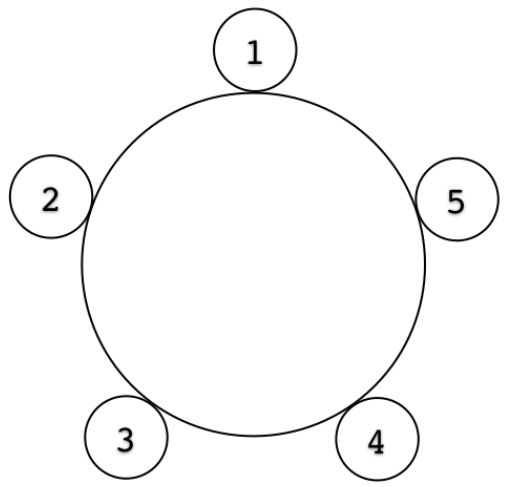
\includegraphics[width=0.3\linewidth]{img1.png}
\end{center}

예를 들어, $k=3$인 경우(K 이사장이 3번 요리를 먹는 경우)를 생각해 보면, 회전대를 돌리는 횟수가 최소가 되는 것은 다음과 같은 방법이다.

\begin{itemize}
	\item K 이사장 (1번 위원)이 회전대를 시계방향으로 두 번 돌려서, 3번 요리를 먹는다.
	\item 3번 위원이 회전대를 돌리지 않고 5번 요리를 먹는다.
	\item 5번 위원이 회전대를 돌리지 않고 5번 요리를 먹는다.
	\item 2번 위원이 회전대를 반시계방향으로 한 번 돌려서, 3번 요리를 먹는다.
	\item 4번 위원이 회전대를 반시계방향으로 두 번 돌려서, 3번 요리를 먹는다.
\end{itemize}


이때 회전대를 돌리는 횟수는 총 $2+1+2=5$ 번이므로, 출력의 세 번째 줄에는 5를 출력한다.



\end{problem}


